\section{Lecture 13: Introduction to Quantum Approximate Optimization
Algorithms (QAOA)}\label{sec:lecture13}

\subsection*{Review}

\qs{VQA}{
  What varies when running a variational quantum algorithm?
}

\sol{
  Rotation gate angles.
}

\qs{Ansatz in QAOA}{
  What does "ansatz" refer to in Quantum Alternating Operator Ansatz (aka QAOA)?
}

\sol{
  Making a guess about the quantum circuit to use for optimization.
}


%%%%%%%%%%%%%%%%%

\index{Quantum Approximate Optimization Algorithms}
\subsection*{Quantum Approximate Optimization Algorithms}
\dfn{Quantum Approximate Optimization Algorithm (QAOA)}{ \textbf{The Quantum
  Approximate Optimization Algorithm (QAOA)} is a hybrid quantum-classical
  algorithm within the Variational Quantum Algorithm (VQA) family, designed
  to approximate solutions to combinatorial optimization problems (e.g.,
  \textsc{Max-Cut}, graph coloring). Introduced by Farhi, Goldstone, and Gutmann,
  \footnote{"A Quantum Approximate Optimization Algorithm":
  \url{https://arxiv.org/abs/1411.4028}} QAOA uses a parameterized quantum circuit
  to prepare a state $\ket{\psi(\gamma, \beta)}$ whose expectation value with
  respect to a cost Hamiltonian $H_C$ is minimized via classical optimization.
}

\vspace{0.3cm}

\begin{figure}[H]
  \centering
  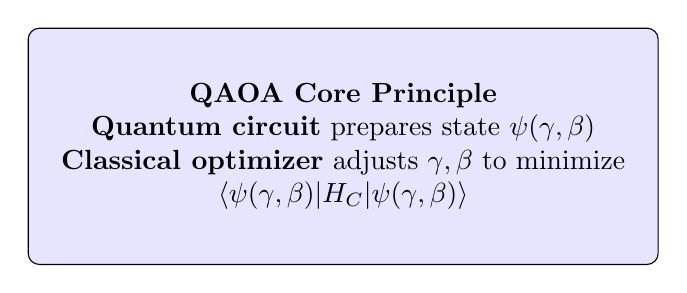
\begin{tikzpicture}
    \node[draw, rounded corners, minimum width=8cm, minimum height=3cm, fill=blue!10] (box) {};
    \node[align=center] at (box.center) {
        \textbf{QAOA Core Principle}\\
        \textbf{Quantum circuit} prepares state $\ket{\psi(\gamma, \beta)}$\\
        \textbf{Classical optimizer} adjusts $\gamma, \beta$ to minimize\\
        $\langle \psi(\gamma, \beta) | H_C | \psi(\gamma, \beta) \rangle$
      };
  \end{tikzpicture}
  \caption{Conceptual view of QAOA as a hybrid quantum-classical algorithm}
  \label{fig:qaoa-principle}
\end{figure}

\noindent
\textbf{Core Ideas:}
\begin{itemize}
  \index{Quantum Approximate Optimization Algorithms!Cost Hamiltonian}
  \item \textbf{Cost Hamiltonian ($H_C$)}: Encodes the problem's objective,
    e.g., $H_C = \sum_{\langle i,j \rangle} Z_i Z_j$ for \textsc{Max-Cut}, where lower
    energy states correspond to better solutions.

    \vspace{0.3cm}

    \index{Quantum Approximate Optimization Algorithms!Mixing Hamiltonian}
  \item \textbf{Mixing Hamiltonian ($H_M$)}: Typically $H_M = \sum_i X_i$,
    drives exploration across the solution space.

    \vspace{0.3cm}

    \index{Quantum Approximate Optimization Algorithms!ansatz}
  \item \textbf{Ansatz State}: $\ket{\psi(\gamma, \beta)} = \prod_{p=1}^P
    e^{-i\beta_p H_M} e^{-i\gamma_p H_C} \ket{s}$, where $\ket{s}$ is a
    uniform superposition (e.g., $H^{\otimes n} \ket{0}^{\otimes n}$), and
    $P$ is the number of layers.

    \vspace{0.3cm}

  \item \boxed{\textbf{Goal}}: Find $\gamma = (\gamma_1, \ldots, \gamma_P)$ and
    $\beta = (\beta_1, \ldots, \beta_P)$ minimizing $\langle \psi(\gamma,
    \beta) | H_C | \psi(\gamma, \beta) \rangle$.

\end{itemize}

\vspace{0.3cm}

\nt{
  QAOA's hybrid nature makes it suitable for Noisy Intermediate-Scale Quantum
  (NISQ) devices, as it relies on shallow circuits and classical feedback loops.
}

\vspace{0.3cm}

\begin{figure}[H]
  \centering
  \begin{tikzpicture}
        % Define the nodes for the flowchart
    \node[draw, rounded corners, fill=green!10] (init) {Initialize qubits in $\ket{s}=H^{\otimes n}\ket{0}^{\otimes n}$};
    \node[draw, rounded corners, fill=orange!10, below=0.5cm of init] (cost) {Apply cost unitary $e^{-i\gamma_p H_C}$};
    \node[draw, rounded corners, fill=blue!10, below=0.5cm of cost] (mix) {Apply mixing unitary $e^{-i\beta_p H_M}$};
    \node[draw, rounded corners, fill=red!10, below=0.5cm of mix] (meas) {Measure in computational basis};
    \node[draw, rounded corners, fill=purple!10, below=0.5cm of meas] (opt) {Optimize parameters $\gamma, \beta$};

        % Draw the arrows
    \draw[->, thick] (init) -- (cost);
    \draw[->, thick] (cost) -- (mix);
    \draw[->, thick] (mix) -- (meas);
    \draw[->, thick] (meas) -- (opt);
    \draw[->, thick] (opt) to[out=180, in=180] node[left] {Repeat} (init);

        % Add a label for the p=1 to P loop
    \draw[rounded corners, dashed] ($(cost.north west)+(-0.3,0.2)$) rectangle ($(mix.south east)+(0.3,-0.2)$);
    \node[right] at ($(mix.east)+(0.4,0)$) {Repeat for $p=1$ to $P$};
  \end{tikzpicture}
  \caption{QAOA algorithm workflow}
  \label{fig:qaoa-workflow}
\end{figure}

\noindent
\textbf{Algorithm Steps:}
\begin{enumerate}
  \item \textbf{Initialize}: For $n$ qubits, apply Hadamard gates: $\ket{s} =
    H^{\otimes n} \ket{0}^{\otimes n} = \frac{1}{\sqrt{2^n}} \sum_{x \in
    \{0,1\}^n} \ket{x}$.

  \item \textbf{Apply Ansatz}: For $p=1$ to $P$, apply $e^{-i\gamma_p H_C}$
    (cost evolution) followed by $e^{-i\beta_p H_M}$ (mixing evolution).

  \item \textbf{Measure}: Compute $\langle H_C \rangle$ by measuring in the
    computational basis and calculating the expectation value.

  \item \textbf{Optimize}: Use a classical algorithm (e.g., gradient descent,
    BFGS, Nelder-Mead) to adjust $\gamma_p$ and $\beta_p$ parameters.

  \item \textbf{Repeat}: Iterate until $\langle H_C \rangle$ converges to an
    approximate minimum or a set number of iterations is reached.

\end{enumerate}

\subsubsection*{\textsc{Max-Cut} Example}

\textsc{Max-Cut} is a classic combinatorial optimization problem where we aim
to partition graph vertices into two sets, maximizing the number (or weight)
of edges crossing between the sets.

\begin{figure}[H]
  \centering
  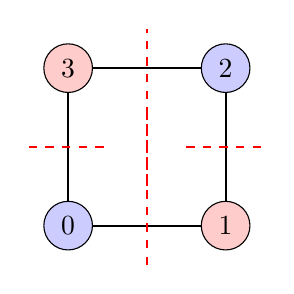
\begin{tikzpicture}
        % Draw the nodes of the cycle graph
    \node[circle, draw, fill=blue!20] (0) at (0,0) {0};
    \node[circle, draw, fill=red!20] (1) at (2,0) {1};
    \node[circle, draw, fill=blue!20] (2) at (2,2) {2};
    \node[circle, draw, fill=red!20] (3) at (0,2) {3};

        % Draw the edges
    \draw[thick] (0) -- (1);
    \draw[thick] (1) -- (2);
    \draw[thick] (2) -- (3);
    \draw[thick] (3) -- (0);

        % Show the cut
    \draw[dashed, red, thick] (1,0.5) -- (1,1.5);
    \draw[dashed, red, thick] (-0.5,1) -- (0.5,1);
    \draw[dashed, red, thick] (1.5,1) -- (2.5,1);
    \draw[dashed, red, thick] (1,-0.5) -- (1,2.5);
  \end{tikzpicture}
  \caption{A 4-node cycle graph with an optimal \textsc{Max-Cut} solution (nodes
  colored by partition)}
  \label{fig:max-cut-example}
\end{figure}

Consider a 4-node cycle graph with edges $\{(0,1), (1,2), (2,3), (3,0)\}$ and
weights $w_{ij} = 1$. The \textsc{Max-Cut} problem seeks a partition maximizing cut
edges.

\vspace{0.3cm}

\noindent
\textbf{Cost Hamiltonian:}

\vspace{0.3cm}

For the \textsc{Max-Cut} problem, the cost Hamiltonian is constructed as:
\[
  H_C = \sum_{\langle i,j \rangle} \frac{1 - Z_i Z_j}{2} = \text{constant} -
  \frac{1}{2}\sum_{\langle i,j \rangle} Z_i Z_j
\]

For our 4-node cycle graph, this becomes:
\[
  H_C = 2 - \frac{1}{2}(Z_0 Z_1 + Z_1 Z_2 + Z_2 Z_3 + Z_3 Z_0)
\]

Since the constant term doesn't affect optimization, we typically use:
\[
  H_C \propto -(Z_0 Z_1 + Z_1 Z_2 + Z_2 Z_3 + Z_3 Z_0)
\]

Eigenstate $\ket{0101}$ (alternating partition) has eigenvalue $-4$
(corresponding to 4 cuts, which is optimal).

\vspace{0.3cm}

\noindent
\textbf{Mixing Hamiltonian:}
\[
  H_M = X_0 + X_1 + X_2 + X_3
\]

\vspace{0.3cm}

The mixing Hamiltonian generates transitions between computational basis
states, enabling exploration of the solution space.

\vspace{0.3cm}

\noindent
\textbf{QAOA Circuit Implementation ($P=1$):}

\begin{figure}[H]
  \centering
  \begin{quantikz}
    \lstick{$q_0: \ket{0}$} & \gate{H} & \ctrl{1} & \qw & \ctrl{1} & \qw & \ctrl{3} & \qw & \ctrl{3} & \qw & \gate{R_X(2\beta)} & \meter{} \\
    \lstick{$q_1: \ket{0}$} & \gate{H} & \targ{} & \gate{R_Z(2\gamma)} & \targ{} & \ctrl{1} & \qw & \qw & \qw & \qw & \gate{R_X(2\beta)} & \meter{} \\
    \lstick{$q_2: \ket{0}$} & \gate{H} & \qw & \qw & \qw & \targ{} & \qw & \gate{R_Z(2\gamma)} & \qw & \ctrl{1} & \gate{R_X(2\beta)} & \meter{} \\
    \lstick{$q_3: \ket{0}$} & \gate{H} & \qw & \qw & \qw & \qw & \targ{} & \qw & \targ{} & \targ{} & \gate{R_X(2\beta)} & \meter{} \\
  \end{quantikz}
  \caption{Detailed QAOA circuit for the 4-node \textsc{Max-Cut} problem with $P=1$}
  \label{fig:detailed-qaoa-circuit}
\end{figure}

\begin{itemize}
  \item \textbf{Implementing $e^{-i\gamma Z_i Z_j}$}:
    We use CNOTs and $R_Z(2\gamma)$ gates, since $e^{-i\gamma Z_i Z_j} = \text{CNOT}_{i,j} \cdot (I \otimes R_Z(2\gamma)) \cdot \text{CNOT}_{i,j}$.

  \item \textbf{Implementing $e^{-i\beta X_i}$}:
    We can directly implement this with $R_X(2\beta)$ rotation gates.
\end{itemize}

\vspace{0.3cm}

\ex{Simplified \textsc{Max-Cut} Circuit ($P=1$)}{
  The QAOA ansatz for $P=1$ can be represented at a higher level as:
  \[
    \begin{quantikz}
      \lstick{$q_0: \ket{0}$} & \gate{H} & \gate{e^{-i\gamma Z_0 Z_1}} & \gate{e^{-i\gamma Z_3 Z_0}} & \gate{R_X(2\beta)} & \meter{} \\
      \lstick{$q_1: \ket{0}$} & \gate{H} & \gate{e^{-i\gamma Z_1 Z_2}} & \qw & \gate{R_X(2\beta)} & \meter{} \\
      \lstick{$q_2: \ket{0}$} & \gate{H} & \qw & \gate{e^{-i\gamma Z_2 Z_3}} & \gate{R_X(2\beta)} & \meter{} \\
      \lstick{$q_3: \ket{0}$} & \gate{H} & \qw & \qw & \gate{R_X(2\beta)} & \meter{}
    \end{quantikz}
  \]

  This structure clearly shows the alternating pattern of cost evolution
  ($e^{-i\gamma Z_i Z_j}$ gates) followed by mixing evolution ($R_X(2\beta)$
  gates).
}

\subsubsection*{Circuit Implementation in Cirq}

Here's a complete QAOA circuit for the 4-qubit \textsc{Max-Cut} with $P=1$ using
Google's \texttt{Cirq} framework:

\begin{minted}[linenos]{python}
import cirq
import numpy as np
import matplotlib.pyplot as plt
from scipy.optimize import minimize

# Define the 4-node cycle graph
def get_graph():
    edges = [(0, 1), (1, 2), (2, 3), (3, 0)]
    return edges

# Create QAOA circuit for Max-Cut
def create_qaoa_circuit(qubits, edges, gamma, beta):
    circuit = cirq.Circuit()

    # Initialize with Hadamard gates
    circuit.append(cirq.H.on_each(qubits))

    # Apply cost Hamiltonian
    for i, j in edges:
        circuit.append(cirq.ZZPowGate(exponent=2*gamma/np.pi).on(qubits[i], qubits[j]))

    # Apply mixing Hamiltonian
    circuit.append(cirq.rx(2*beta).on_each(qubits))

    return circuit

# Calculate Max-Cut expectation value from bitstring
def calculate_cut_value(bitstring, edges):
    cut_value = 0
    for i, j in edges:
        if bitstring[i] != bitstring[j]:
            cut_value += 1
    return cut_value

# Main QAOA function
def run_qaoa_max_cut(gamma, beta, num_qubits=4, shots=8192):
    qubits = cirq.LineQubit.range(num_qubits)
    edges = get_graph()

    # Create and run the circuit
    circuit = create_qaoa_circuit(qubits, edges, gamma, beta)
    measurement_circuit = circuit + cirq.measure(*qubits, key='result')

    # Simulate
    simulator = cirq.Simulator()
    result = simulator.run(measurement_circuit, repetitions=shots)

    # Process results
    counts = result.histogram(key='result')

    # Calculate expected cut value
    expectation = 0
    total_samples = sum(counts.values())

    for bitstring, count in counts.items():
        # Convert integer to binary representation
        binary = format(bitstring, f'0{num_qubits}b')
        cut_val = calculate_cut_value([int(bit) for bit in binary], edges)
        expectation += cut_val * (count / total_samples)

    return -expectation  # Negative since we're minimizing

# Optimize parameters
def optimize_qaoa():
    # Initial parameters
    initial_params = [0.5, 0.5]  # [gamma, beta]

    # Perform optimization
    result = minimize(
        lambda params: run_qaoa_max_cut(params[0], params[1]),
        initial_params,
        method='COBYLA',
        options={'maxiter': 100}
    )

    # Return optimized parameters
    return result.x

# Execute full QAOA
gamma_opt, beta_opt = optimize_qaoa()
circuit = create_qaoa_circuit(cirq.LineQubit.range(4), get_graph(), gamma_opt, beta_opt)
print(f"Optimized parameters: gamma={gamma_opt}, beta={beta_opt}")
print(f"Estimated Max-Cut: {-run_qaoa_max_cut(gamma_opt, beta_opt)}")
\end{minted}

%%%%%%%%%%%

\noindent
\index{Quantum Approximate Optimization Algorithms!advantages@\textit{advantages}}
\textbf{QAOA Advantages}
\begin{itemize}
  \item \textbf{NISQ Compatibility}: QAOA uses shallow circuits (small
    $P$), making it feasible on current noisy quantum hardware without error
    correction.

  \item \textbf{Theoretical Guarantees}: For $P \to \infty$, QAOA approaches
    the exact solution, resembling adiabatic quantum
    computation\footnote{Farhi et al. demonstrated that QAOA with $P \to
    \infty$ converges to the adiabatic quantum algorithm, which provides a
  theoretical foundation for QAOA's potential quantum advantage.}.

  \item \textbf{Problem Flexibility}: Can be adapted to many NP-hard problems
    by appropriate encoding of the cost Hamiltonian.

\end{itemize}


\aside{
  The connection to adiabatic computation suggests QAOA's theoretical power,
  but practical limits (e.g., noise, coherence time) often restrict $P$ to
  small values in current hardware.
}

\vspace{0.3cm}

\begin{figure}[H]
  \centering
  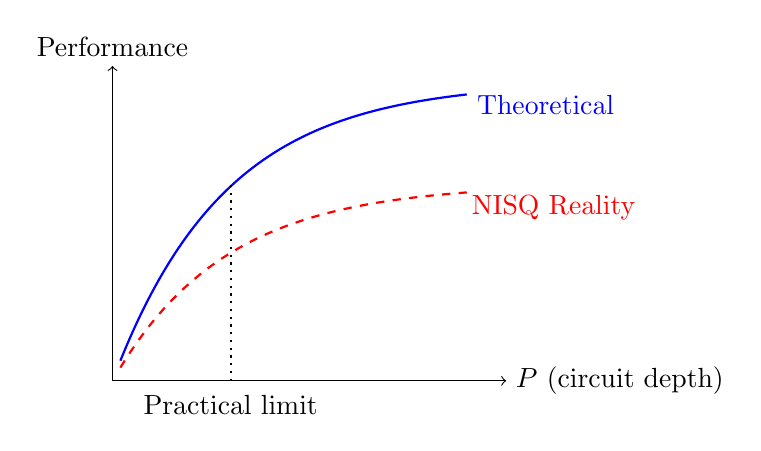
\begin{tikzpicture}
        % Draw axes
    \draw[->] (0,0) -- (5,0) node[right] {$P$ (circuit depth)};
    \draw[->] (0,0) -- (0,4) node[above] {Performance};

        % Draw curves
    \draw[blue, thick, domain=0.1:4.5, samples=100] plot (\x, {3.8*(1-exp(-0.7*\x))});
    \draw[red, dashed, thick, domain=0.1:4.5, samples=100] plot (\x, {2.5*(1-exp(-0.7*\x))});

        % Add labels
    \node[blue] at (5.5,3.5) {Theoretical};
    \node[red] at (5.6,2.2) {NISQ Reality};

        % Add a vertical line showing practical limit
    \draw[dotted, thick] (1.5,0) -- (1.5,2.5);
    \node at (1.5,-0.3) {Practical limit};
  \end{tikzpicture}
  \caption{Theoretical vs. practical QAOA performance as function of circuit
  depth $P$}
  \label{fig:qaoa-performance}
\end{figure}

\noindent
\index{Quantum Approximate Optimization Algorithms!limitations@\textit{limitations}}
\textbf{QAOA Limitations}

\begin{itemize}
  \item \textbf{Barren Plateaus}: For large problem sizes, the optimization
    landscape can become exponentially flat in certain regions, making it
    difficult for classical optimizers to find good
    parameters\footnote{McClean et al., "Barren plateaus in quantum neural
    network training landscapes", \url{https://arxiv.org/abs/1803.11173}}.

  \item \textbf{Unproven Quantum Advantage}: No guaranteed polynomial speedup
    over classical algorithms has been proven for general cases; performance
    depends on the specific problem instance and $P$.

  \item \textbf{Parameter Optimization Challenges}: Finding optimal $\gamma$
    and $\beta$ parameters becomes increasingly difficult as $P$ and problem
    size grow.
\end{itemize}


%%%%%%%%%%%%%%%%%%%%%%%%%%%%%%%%%%%%%%%%%%%%%%
% End of Lecture 13
%%%%%%%%%%%%%%%%%%%%%%%%%%%%%%%%%%%%%%%%%%%%%%
